\documentclass[man,12pt,floatsintext,donotrepeattitle]{apa7}

\usepackage{latexml}  % \iflatexml: true under LaTeXML/oxide, false under pdflatex
\usepackage[american]{babel}
\usepackage{csquotes}
\usepackage{amsmath,amssymb}
\usepackage{booktabs}
\usepackage{xcolor}
\usepackage[most]{tcolorbox}
\usepackage[style=apa,backend=biber]{biblatex}
\usepackage{xr}
\externaldocument{draft6}
\addbibresource{refs.bib}
\hypersetup{
  hidelinks,
  pdftitle={Supplement 3: Additional Figures},
  pdfauthor={Joseph Corneli},
  pdfsubject={Additional figures accompanying Rule-Rewriting Cellular Automata
    and the Edge of Chaos}
}

\newcommand{\sig}{\sigma}
\newcommand{\bit}[1]{\mathrm{bit}[#1]}
% Cross-reference a finding box by its label (tcolorbox auto counter supplies the number).
\newcommand{\findref}[1]{Box~\ref{#1}}

% Typed boxes are tcolorboxes (TikZ drawings); a converter would render them
% as fixed-geometry SVG rather than text. Define semantic equivalents instead.
% NB: \newif must sit outside the guard -- TeX counts \if tokens when skipping.
\newif\ifpaperboxfold
\iflatexml
  % html-boxes.tex -- converter-side definitions of the paper's typed boxes.
%
% WHY: the print versions of these boxes are tcolorboxes, which are drawn with
% TikZ. latexml-oxide converts TikZ faithfully -- by rendering it as SVG. That
% turns 94% of Supplement 1 and 72% of Supplement 2 into fixed-geometry
% pictures: they do not reflow, they do not scale to a narrow screen, and the
% text inside them is not HTML.
%
% So under a converter we skip tcolorbox entirely and define the same
% environments as ordinary theorem-like blocks. LaTeXML and oxide both emit
% these as <div class="ltx_theorem ltx_theorem_NAME"> with a real title, a real
% counter and a real anchor -- semantic HTML that reflows and can be styled.
%
% Input this from inside an \iflatexml branch, then declare the boxes the
% document actually uses:
%
%     \iflatexml
%       % html-boxes.tex -- converter-side definitions of the paper's typed boxes.
%
% WHY: the print versions of these boxes are tcolorboxes, which are drawn with
% TikZ. latexml-oxide converts TikZ faithfully -- by rendering it as SVG. That
% turns 94% of Supplement 1 and 72% of Supplement 2 into fixed-geometry
% pictures: they do not reflow, they do not scale to a narrow screen, and the
% text inside them is not HTML.
%
% So under a converter we skip tcolorbox entirely and define the same
% environments as ordinary theorem-like blocks. LaTeXML and oxide both emit
% these as <div class="ltx_theorem ltx_theorem_NAME"> with a real title, a real
% counter and a real anchor -- semantic HTML that reflows and can be styled.
%
% Input this from inside an \iflatexml branch, then declare the boxes the
% document actually uses:
%
%     \iflatexml
%       % html-boxes.tex -- converter-side definitions of the paper's typed boxes.
%
% WHY: the print versions of these boxes are tcolorboxes, which are drawn with
% TikZ. latexml-oxide converts TikZ faithfully -- by rendering it as SVG. That
% turns 94% of Supplement 1 and 72% of Supplement 2 into fixed-geometry
% pictures: they do not reflow, they do not scale to a narrow screen, and the
% text inside them is not HTML.
%
% So under a converter we skip tcolorbox entirely and define the same
% environments as ordinary theorem-like blocks. LaTeXML and oxide both emit
% these as <div class="ltx_theorem ltx_theorem_NAME"> with a real title, a real
% counter and a real anchor -- semantic HTML that reflows and can be styled.
%
% Input this from inside an \iflatexml branch, then declare the boxes the
% document actually uses:
%
%     \iflatexml
%       \input{html-boxes}
%       \NewHTMLBox{definition}{Definition}{1}   % 1 = takes a {title} argument
%       \NewHTMLBox{theorem}{Theorem}{0}         % 0 = no title argument
%     \else
%       ... the tcolorbox definitions ...
%     \fi
%
% The [label={...}] option each box carries in the sources is honoured, so
% \ref and \autoref into the boxes keep working.

\usepackage{amsthm}
\usepackage{keyval}

% This file is \input, not a package, so `@` is not a letter here: everything
% touching \define@key or \@empty must sit inside \makeatletter.
\makeatletter

% Option keys. Only `label` does anything; the rest are print-layout keys that
% appear in the sources (fold, breakable=false) and must be absorbed silently.
\define@key{htmlbox}{label}{\def\htmlboxlabel{#1}}
\define@key{htmlbox}{fold}[]{}
\define@key{htmlbox}{unfold}[]{}
\define@key{htmlbox}{breakable}[]{}

\newcommand{\htmlboxsetup}[1]{%
  \def\htmlboxlabel{}%
  \def\htmlbox@opts{#1}%
  \ifx\htmlbox@opts\@empty\else\setkeys{htmlbox}{#1}\fi
  \ifx\htmlboxlabel\@empty\else\expandafter\label\expandafter{\htmlboxlabel}\fi}
\makeatother

% \NewHTMLBox{envname}{Heading}{1 if it takes a mandatory {title}, else 0}
\newcommand{\NewHTMLBox}[3]{%
  % amsthm's default `plain' style italicises the body, which is wrong for
  % findings and worked examples that are pages of prose. `definition' style
  % keeps the body upright and only bolds the heading.
  \theoremstyle{definition}%
  \newtheorem{htmlbox#1}{#2}%
  \ifnum#3=1\relax
    \NewDocumentEnvironment{#1}{O{} m}%
      {\begin{htmlbox#1}[##2]\htmlboxsetup{##1}}%
      {\end{htmlbox#1}}%
  \else
    \NewDocumentEnvironment{#1}{O{}}%
      {\begin{htmlbox#1}\htmlboxsetup{##1}}%
      {\end{htmlbox#1}}%
  \fi}

% Present in the print branch; harmless no-ops here so stray uses do not break.
\providecommand{\foldmark}{}
\providecommand{\thetcbcounter}{}
\makeatletter
\@ifundefined{ifpaperboxfold}{\newif\ifpaperboxfold}{}
\makeatother
\endinput

%       \NewHTMLBox{definition}{Definition}{1}   % 1 = takes a {title} argument
%       \NewHTMLBox{theorem}{Theorem}{0}         % 0 = no title argument
%     \else
%       ... the tcolorbox definitions ...
%     \fi
%
% The [label={...}] option each box carries in the sources is honoured, so
% \ref and \autoref into the boxes keep working.

\usepackage{amsthm}
\usepackage{keyval}

% This file is \input, not a package, so `@` is not a letter here: everything
% touching \define@key or \@empty must sit inside \makeatletter.
\makeatletter

% Option keys. Only `label` does anything; the rest are print-layout keys that
% appear in the sources (fold, breakable=false) and must be absorbed silently.
\define@key{htmlbox}{label}{\def\htmlboxlabel{#1}}
\define@key{htmlbox}{fold}[]{}
\define@key{htmlbox}{unfold}[]{}
\define@key{htmlbox}{breakable}[]{}

\newcommand{\htmlboxsetup}[1]{%
  \def\htmlboxlabel{}%
  \def\htmlbox@opts{#1}%
  \ifx\htmlbox@opts\@empty\else\setkeys{htmlbox}{#1}\fi
  \ifx\htmlboxlabel\@empty\else\expandafter\label\expandafter{\htmlboxlabel}\fi}
\makeatother

% \NewHTMLBox{envname}{Heading}{1 if it takes a mandatory {title}, else 0}
\newcommand{\NewHTMLBox}[3]{%
  % amsthm's default `plain' style italicises the body, which is wrong for
  % findings and worked examples that are pages of prose. `definition' style
  % keeps the body upright and only bolds the heading.
  \theoremstyle{definition}%
  \newtheorem{htmlbox#1}{#2}%
  \ifnum#3=1\relax
    \NewDocumentEnvironment{#1}{O{} m}%
      {\begin{htmlbox#1}[##2]\htmlboxsetup{##1}}%
      {\end{htmlbox#1}}%
  \else
    \NewDocumentEnvironment{#1}{O{}}%
      {\begin{htmlbox#1}\htmlboxsetup{##1}}%
      {\end{htmlbox#1}}%
  \fi}

% Present in the print branch; harmless no-ops here so stray uses do not break.
\providecommand{\foldmark}{}
\providecommand{\thetcbcounter}{}
\makeatletter
\@ifundefined{ifpaperboxfold}{\newif\ifpaperboxfold}{}
\makeatother
\endinput

%       \NewHTMLBox{definition}{Definition}{1}   % 1 = takes a {title} argument
%       \NewHTMLBox{theorem}{Theorem}{0}         % 0 = no title argument
%     \else
%       ... the tcolorbox definitions ...
%     \fi
%
% The [label={...}] option each box carries in the sources is honoured, so
% \ref and \autoref into the boxes keep working.

\usepackage{amsthm}
\usepackage{keyval}

% This file is \input, not a package, so `@` is not a letter here: everything
% touching \define@key or \@empty must sit inside \makeatletter.
\makeatletter

% Option keys. Only `label` does anything; the rest are print-layout keys that
% appear in the sources (fold, breakable=false) and must be absorbed silently.
\define@key{htmlbox}{label}{\def\htmlboxlabel{#1}}
\define@key{htmlbox}{fold}[]{}
\define@key{htmlbox}{unfold}[]{}
\define@key{htmlbox}{breakable}[]{}

\newcommand{\htmlboxsetup}[1]{%
  \def\htmlboxlabel{}%
  \def\htmlbox@opts{#1}%
  \ifx\htmlbox@opts\@empty\else\setkeys{htmlbox}{#1}\fi
  \ifx\htmlboxlabel\@empty\else\expandafter\label\expandafter{\htmlboxlabel}\fi}
\makeatother

% \NewHTMLBox{envname}{Heading}{1 if it takes a mandatory {title}, else 0}
\newcommand{\NewHTMLBox}[3]{%
  % amsthm's default `plain' style italicises the body, which is wrong for
  % findings and worked examples that are pages of prose. `definition' style
  % keeps the body upright and only bolds the heading.
  \theoremstyle{definition}%
  \newtheorem{htmlbox#1}{#2}%
  \ifnum#3=1\relax
    \NewDocumentEnvironment{#1}{O{} m}%
      {\begin{htmlbox#1}[##2]\htmlboxsetup{##1}}%
      {\end{htmlbox#1}}%
  \else
    \NewDocumentEnvironment{#1}{O{}}%
      {\begin{htmlbox#1}\htmlboxsetup{##1}}%
      {\end{htmlbox#1}}%
  \fi}

% Present in the print branch; harmless no-ops here so stray uses do not break.
\providecommand{\foldmark}{}
\providecommand{\thetcbcounter}{}
\makeatletter
\@ifundefined{ifpaperboxfold}{\newif\ifpaperboxfold}{}
\makeatother
\endinput

  \NewHTMLBox{empiricalfinding}{Box}{1}
\else
\newtcolorbox[auto counter]{empiricalfinding}[2][]{%
  enhanced,
  breakable,
  colback=orange!7,
  colframe=orange!65!black,
  boxrule=0.7pt,
  arc=1.5mm,
  left=2.5mm,
  right=2.5mm,
  top=1.5mm,
  bottom=1.5mm,
  fonttitle=\bfseries,
  title={Box~\thetcbcounter: #2},
  #1}
\fi

\title{Supplement 3: Additional Figures}
\shorttitle{Additional Figures}
\authorsnames{Joseph Corneli}
\authorsaffiliations{{Oxford Brookes University, Oxford OX3 0BP, United Kingdom},
  {Hyperreal Enterprises Ltd, United Kingdom}}
\note{Supplement to \emph{Rule-Rewriting Cellular Automata and the Edge of
Chaos}. Correspondence: \href{mailto:jcorneli@brookes.ac.uk}
{jcorneli@brookes.ac.uk}.}

\abstract{%
Two survey galleries referred to from the main paper: the rotation-offset sweep
that Part~I classifies, and the spacetime fields behind the diversity mechanisms
of Part~II. Each shows a family of runs at a glance rather than carrying an
argument on its own.}

\renewcommand{\thefigure}{S3.\arabic{figure}}

\begin{document}

\part*{Supplement 3: Additional Figures}

Two survey galleries referred to from the main paper. Each shows a family of runs at a
glance rather than carrying an argument on its own: the first sweeps the rotation
offsets that Part~I classifies, the second shows the spacetime fields behind the
diversity mechanisms of Part~II. They are collected here so the main narrative is not
interrupted by four full pages of plates. Figures~S3.3--S3.7 are measurement
figures relocated from the main paper's ninth draft: the rotation-population
curve, the two-4-cycle contrast, the diversity-control schedule, and the two
damage-sweep panels whose result the main text's placement figure carries.

\begin{figure}[tbp]
\centering
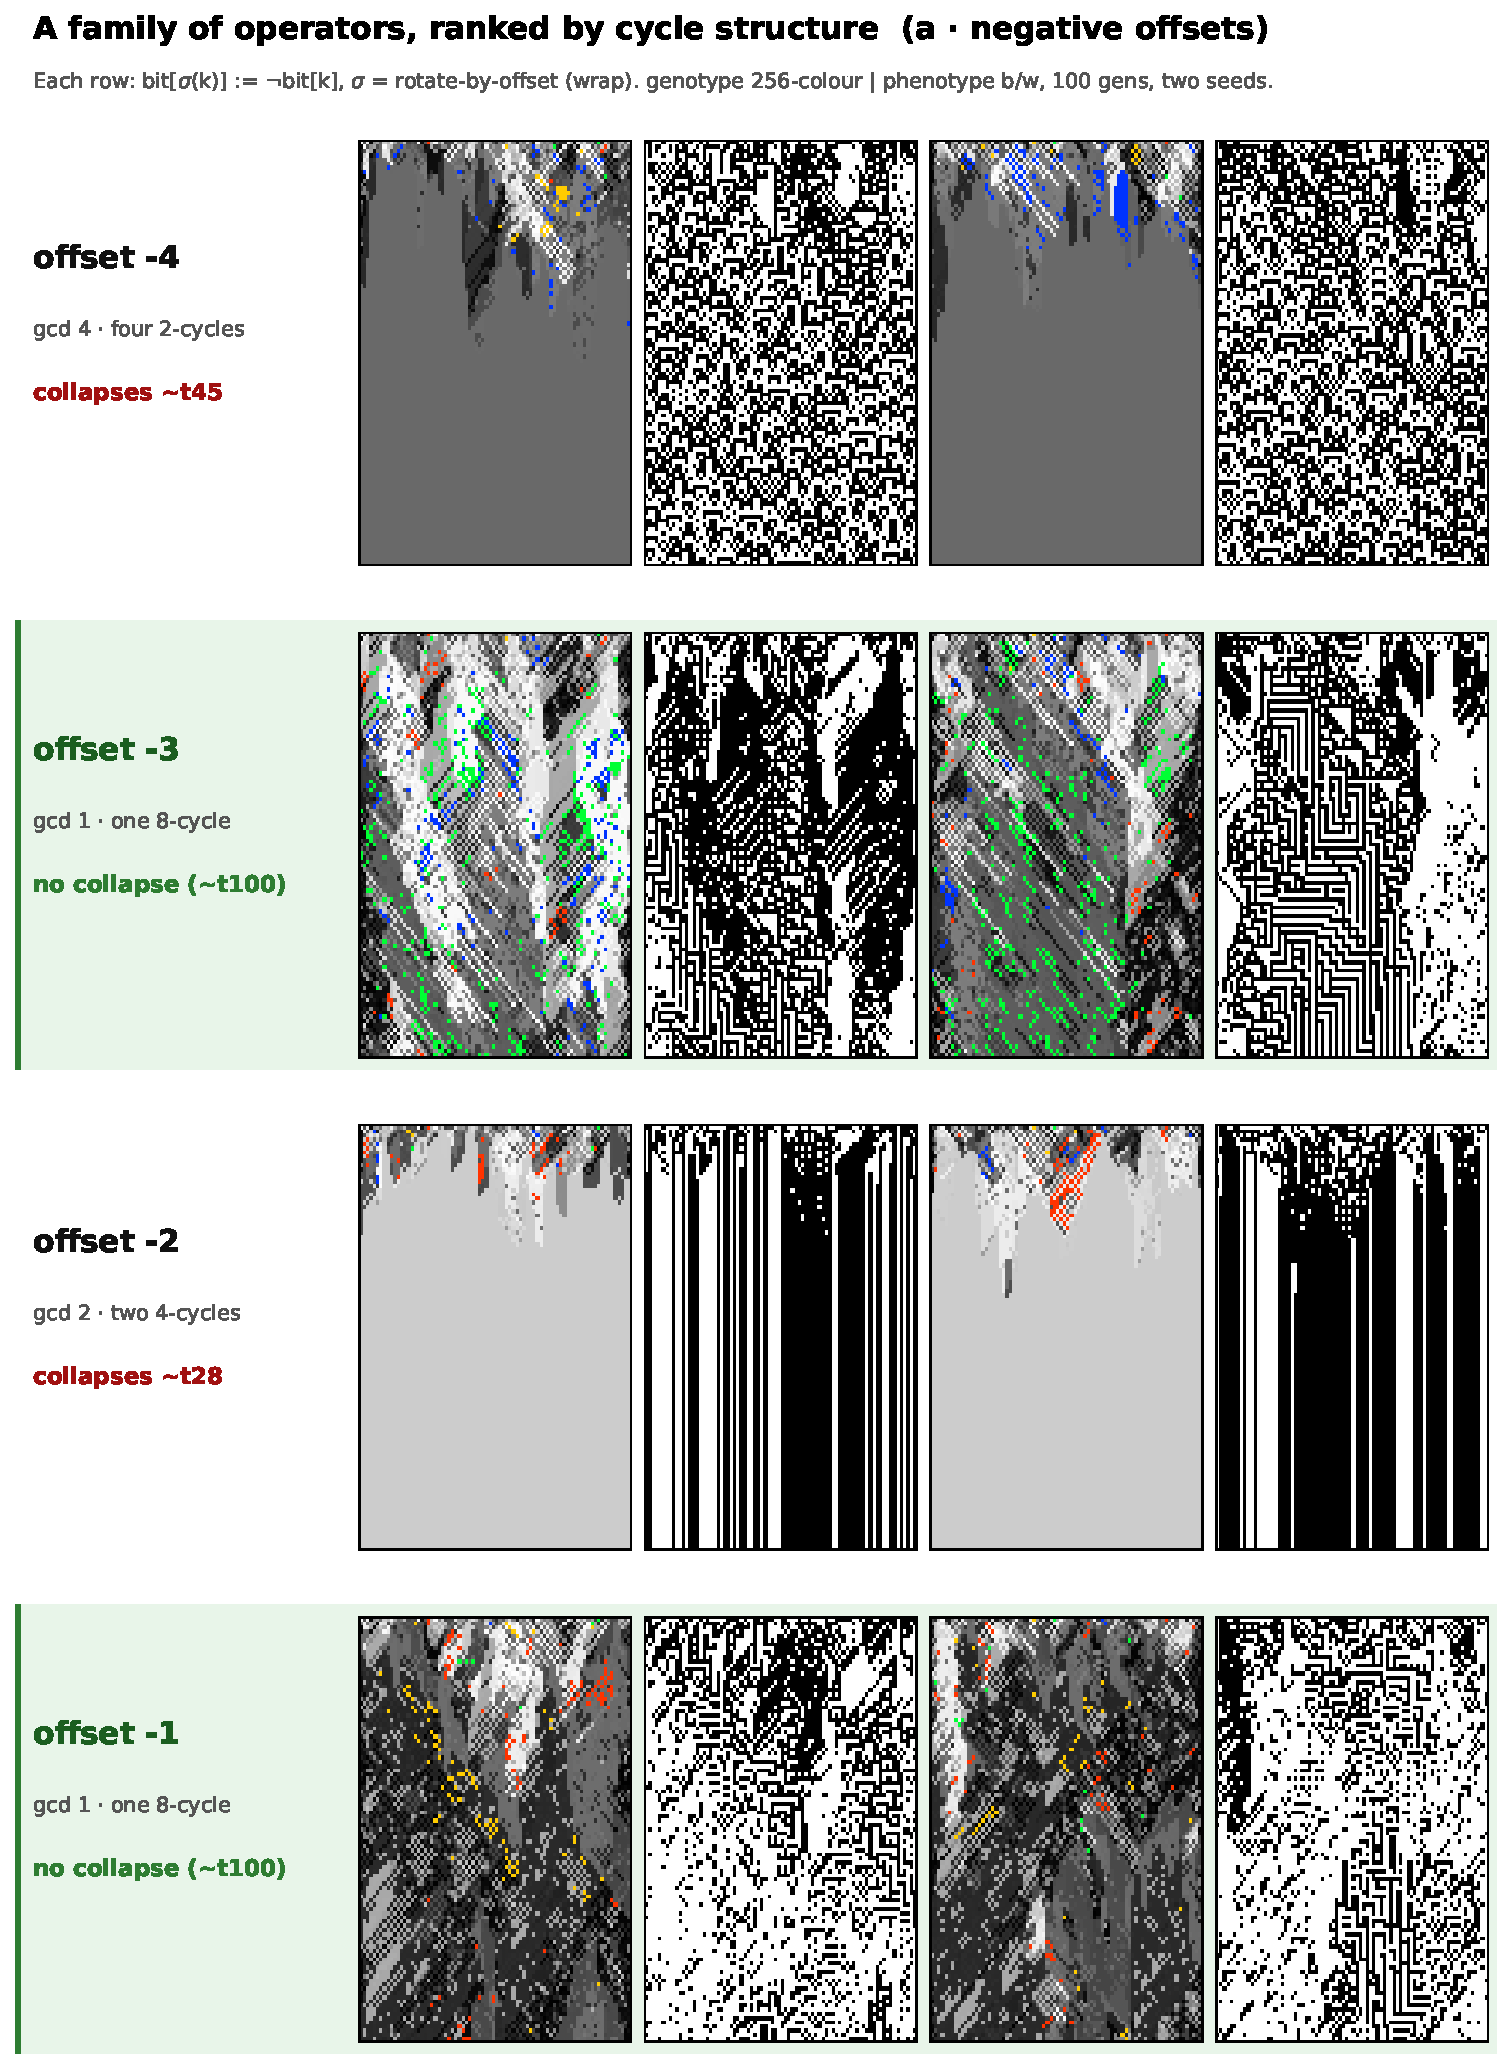
\includegraphics[height=0.73\textheight]{figures/survey_a.pdf}
\caption{\textbf{(a)~Negative offsets.} The rotation subfamily, ordered by
offset: each row is one wrap rotation $\bit{\sig(k)} := \lnot\,\bit{k}$ (two
seeds; genotype in 256 colours, phenotype black and white, first hundred
generations). Of these all-even rotations only the single 8-cycles,
$\gcd(\text{offset},8) = 1$---offset $\pm 1$ and $\pm 3$, highlighted---sustain a
high-diversity phase; offset $\pm 2$ ($\gcd 2$) and $\pm 4$ ($\gcd 4$) collapse.
See Worked Worked example~4; continued in~(b).}
\label{fig:eoc}
\end{figure}

\begin{figure}[tbp]
\ContinuedFloat
\centering
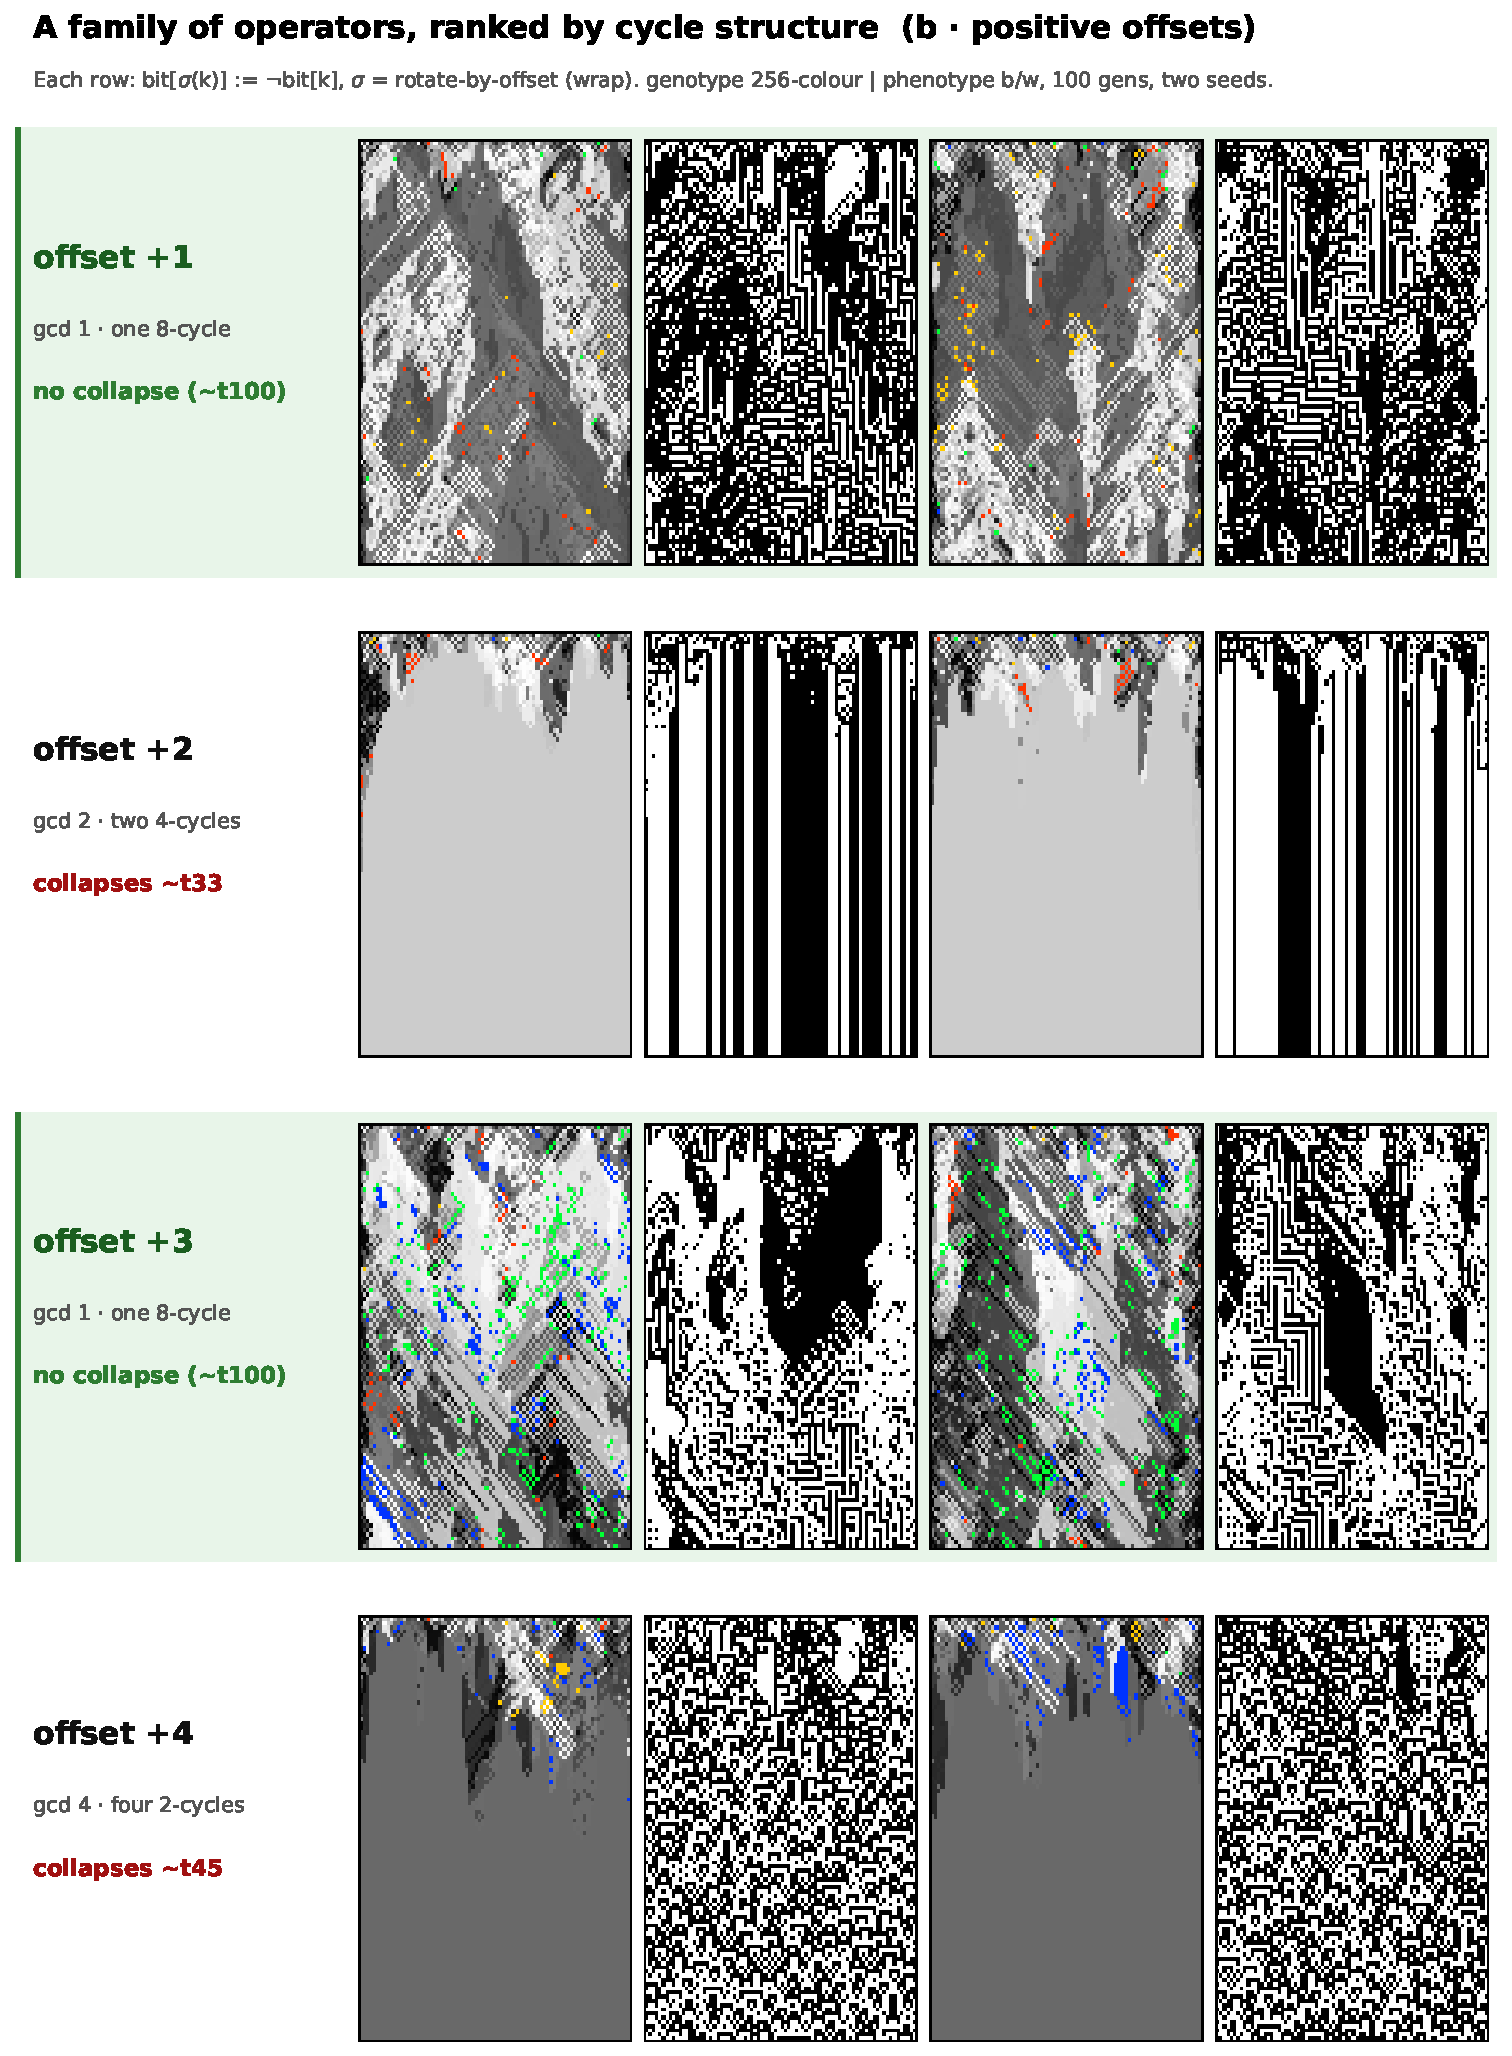
\includegraphics[height=0.73\textheight]{figures/survey_b.pdf}
\caption{\textbf{(b)~Positive offsets.} Continued from~(a). The classification is
symmetric under $d \to -d$ (verdict follows $\gcd(d,8)$), so offset $+1$ sustains
as offset $-1$ does, and offset $+2$ collapses as offset $-2$ does---inverse
rotations sharing verdict but not their transients (Worked
Worked example~4). Possessing a fixed point and staying near it are
different properties: the two pages visually summarise the distinction between
fixed-point existence and spatial persistence.}
\end{figure}

\begin{figure}[tbp]
\centering
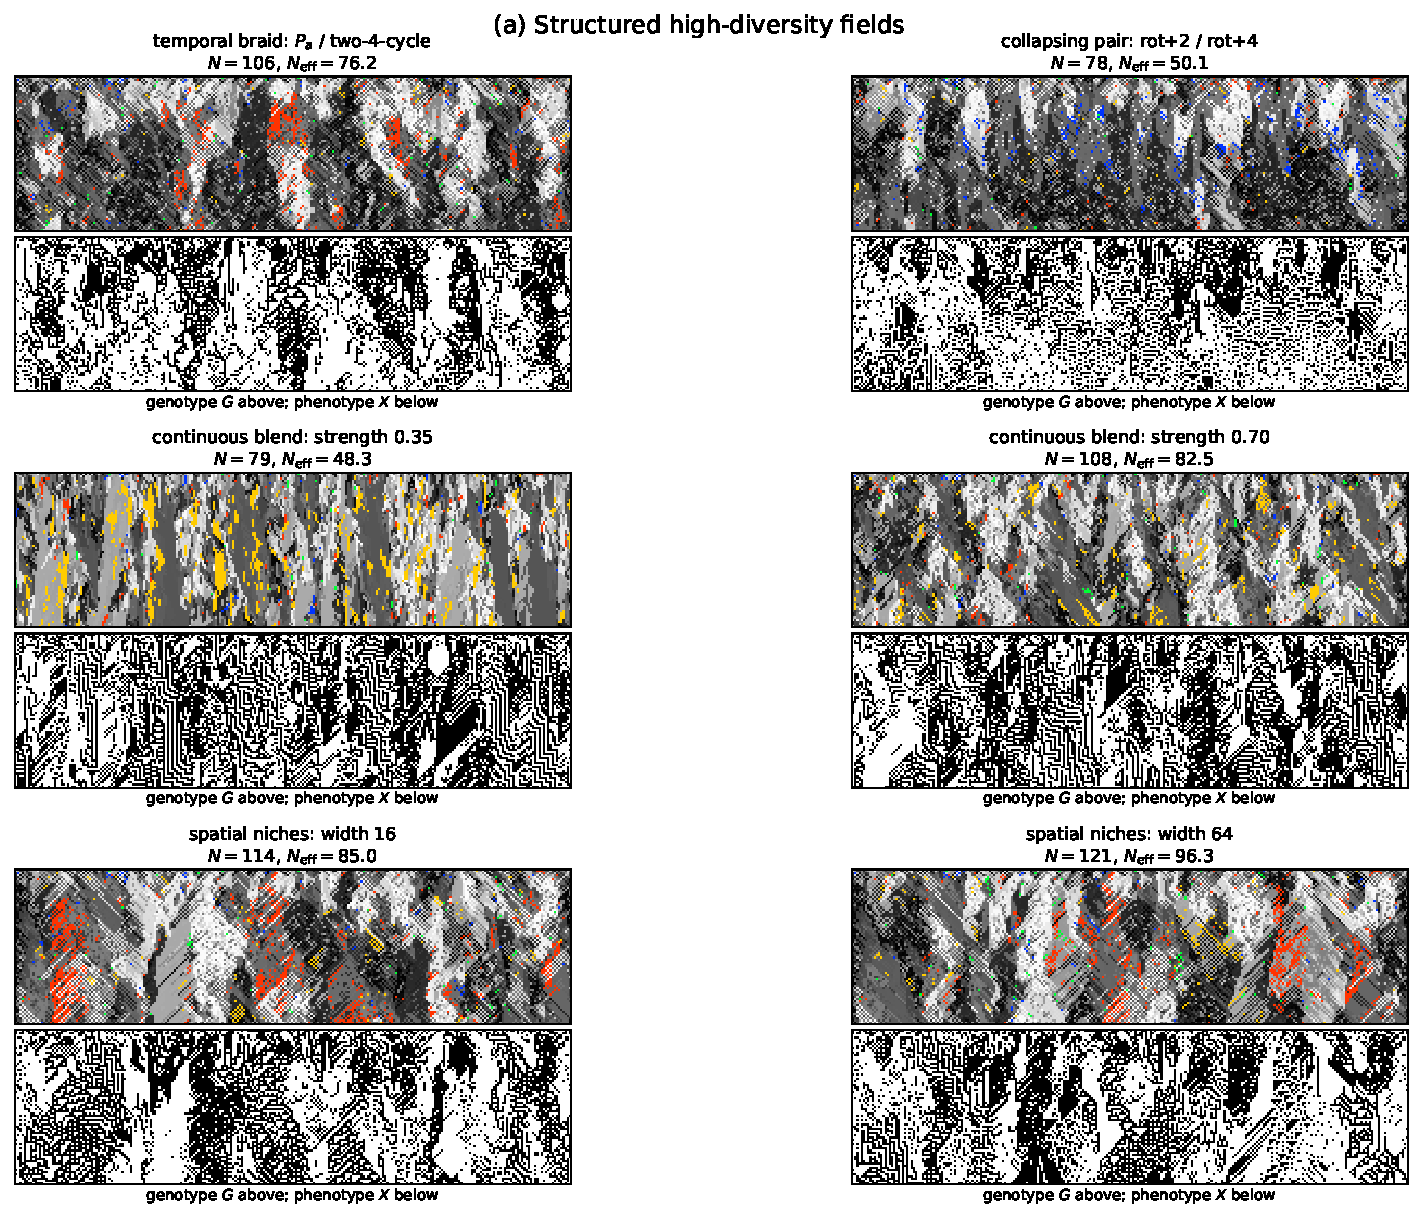
\includegraphics[width=\linewidth]{figures/diversity_spread_a.pdf}
\caption{\textbf{(a)~Structured high-diversity fields.} Six examples from four
mechanism families: temporal alternation; alternation of two operators that
\emph{collapse} when run alone; continuous blending at two strengths; and
spatial niches at two widths. Each tile stacks genotype over phenotype and
reports both distinct-rule and Shannon-effective diversity at $T=70$;
full-population seed $0$, $L=256$. The fields sustain $78$--$121$ rules and
carry coherent diagonal structure at a range of scales. These examples
motivated the candidate diversity coordinate, but the conservative-flow control
in Figure~\ref{fig:diversity-axis} shows that diversity itself does not account
for their propagation.
Continued in~(b).}
\label{fig:diversity-spread}
\end{figure}

\begin{figure}[tbp]
\ContinuedFloat
\centering
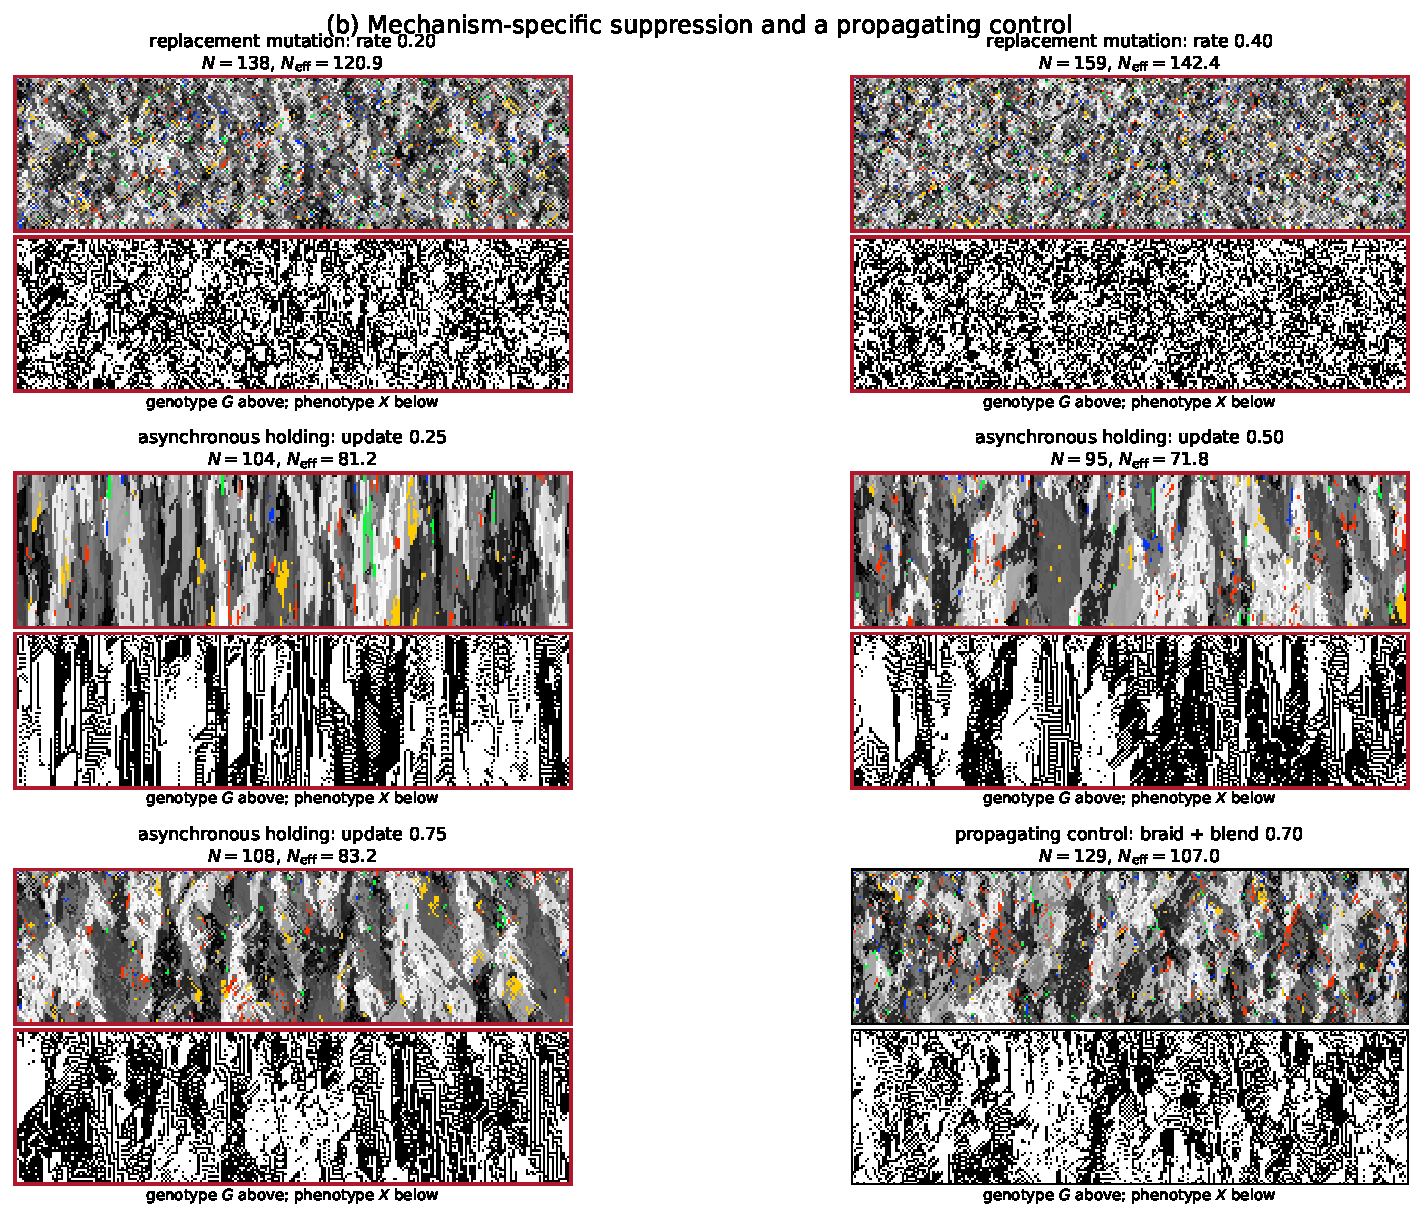
\includegraphics[width=\linewidth]{figures/diversity_spread_b.pdf}
\caption{\textbf{(b)~Two mechanism-specific suppressions.} Continued from~(a);
suppressed configurations are outlined in red. Replacement mutation at rates
$0.20$ and $0.40$ turns the genotype into progressively finer, unstructured
speckle. Asynchronous holding at update fractions $0.25$, $0.50$, and $0.75$
instead produces vertical persistence whose strength changes continuously with
the dial. The unoutlined braid-plus-blend control at bottom right propagates
($3.88$ cells) and recovers the diagonal texture of~(a). The expanded
population makes the distinction visible as a family resemblance rather than a
single selected contrast: these are genuine failure modes of their respective
mechanisms, not evidence for suppression by high diversity.}
\end{figure}

\begin{figure}[t]
\centering
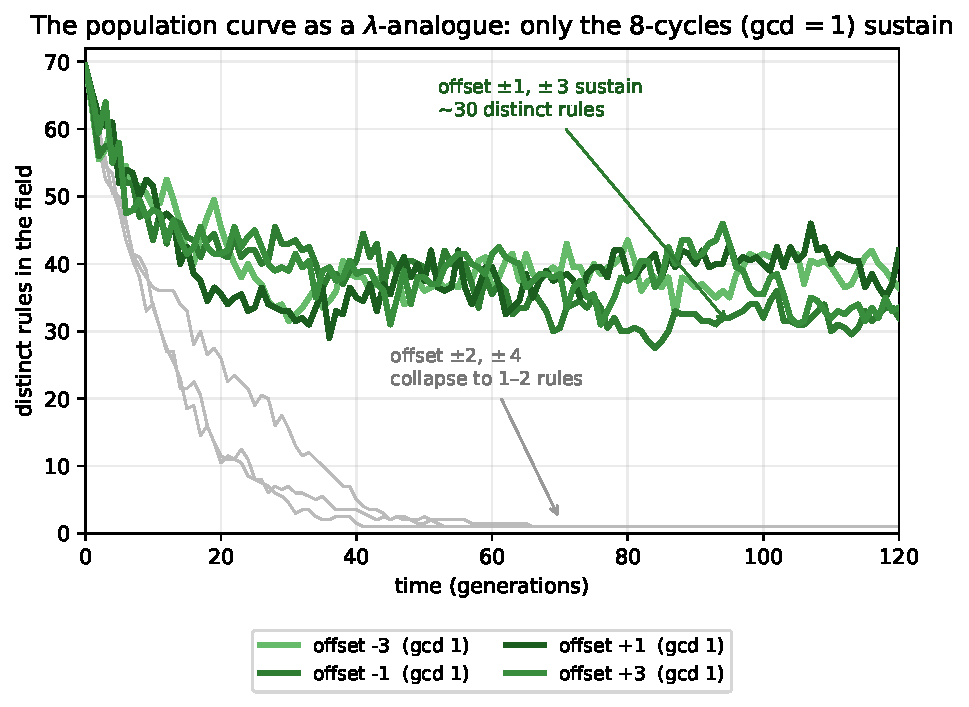
\includegraphics[width=\linewidth]{figures/lambda_analogue.pdf}
\caption{A population observable: distinct rules in the field over time, for
the wrap rotations (two seeds each). All begin at $\approx 70$; the four
8-cycles, $\gcd(\text{offset},8)=1$ (offset $\pm 1$ and $\pm 3$, green), keep a
large diverse population, while offset $\pm 2$ and $\pm 4$ (grey) collapse to one
or two rules. This makes quantitative, on the runs shown, the difference visible
by eye in Figure~S3.1 of this supplement. The main paper's parity-dichotomy figure gives the corresponding
without-blend comparison for offsets $+1$ and $+2$: the former remains active at
lower diversity over that run, while the latter settles onto its four fixed
rules.}
\label{fig:lambda}
\end{figure}

\begin{figure}[t]
\centering
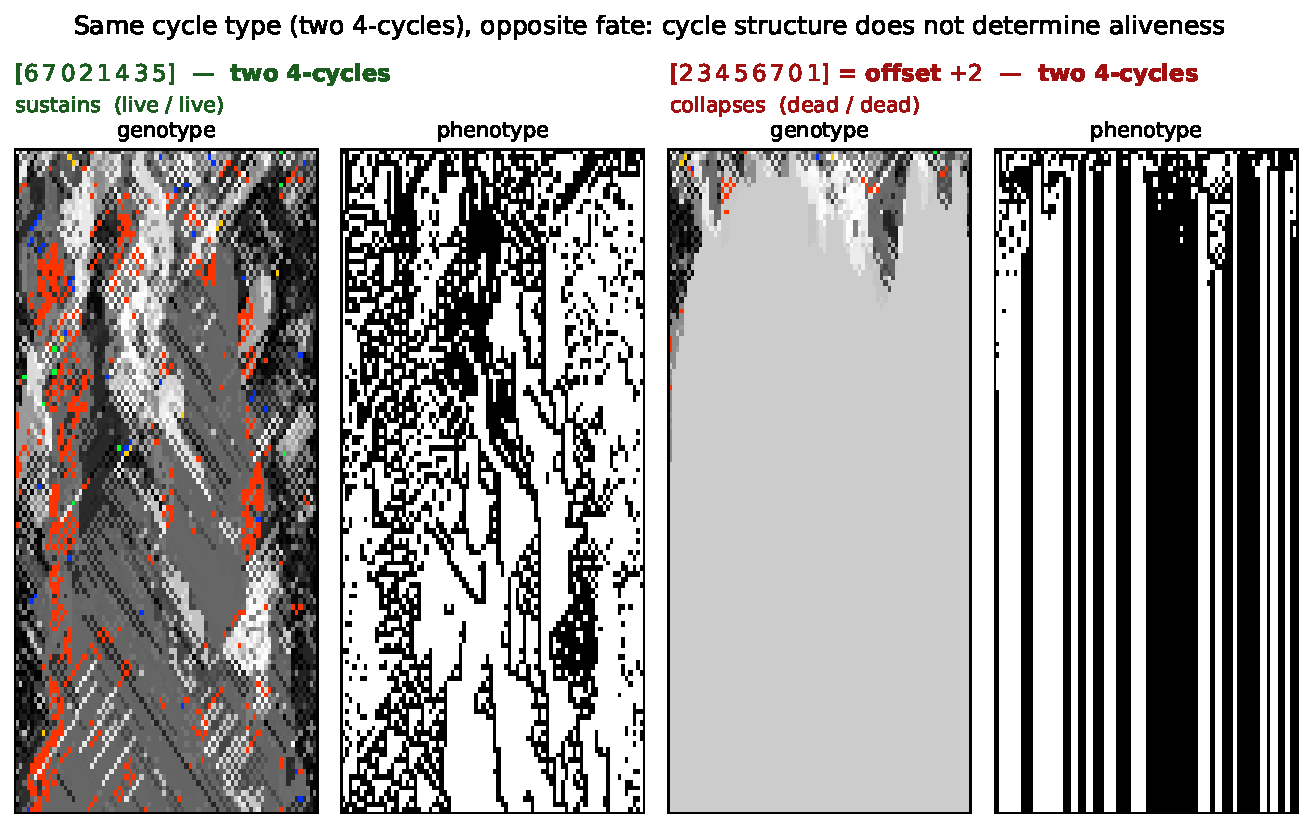
\includegraphics[width=\linewidth]{figures/two4cycle.pdf}
\caption{\textbf{Cycle structure does not determine aliveness.} Two operators of
identical cycle type---both two 4-cycles---with opposite fate. Left,
$[6\,7\,0\,2\,1\,4\,3\,5]$ sustains a live genotype and phenotype; it is the
standard-Wolfram-order form of the historical offset$+2$ operator (its
conjugate). Right, the Wolfram-order rotation offset$+2=[2\,3\,4\,5\,6\,7\,0\,1]$
has the same two-4-cycle structure yet collapses to a dead genotype and a frozen
phenotype. Same cycle type, opposite outcome: the specific permutation, not its
cycle type alone, decides. A full census of the 40320 operators confirms the
two-4-cycle class splits between sustaining and collapsing.}
\label{fig:two4cycle}
\end{figure}

\begin{figure}[t]
\centering
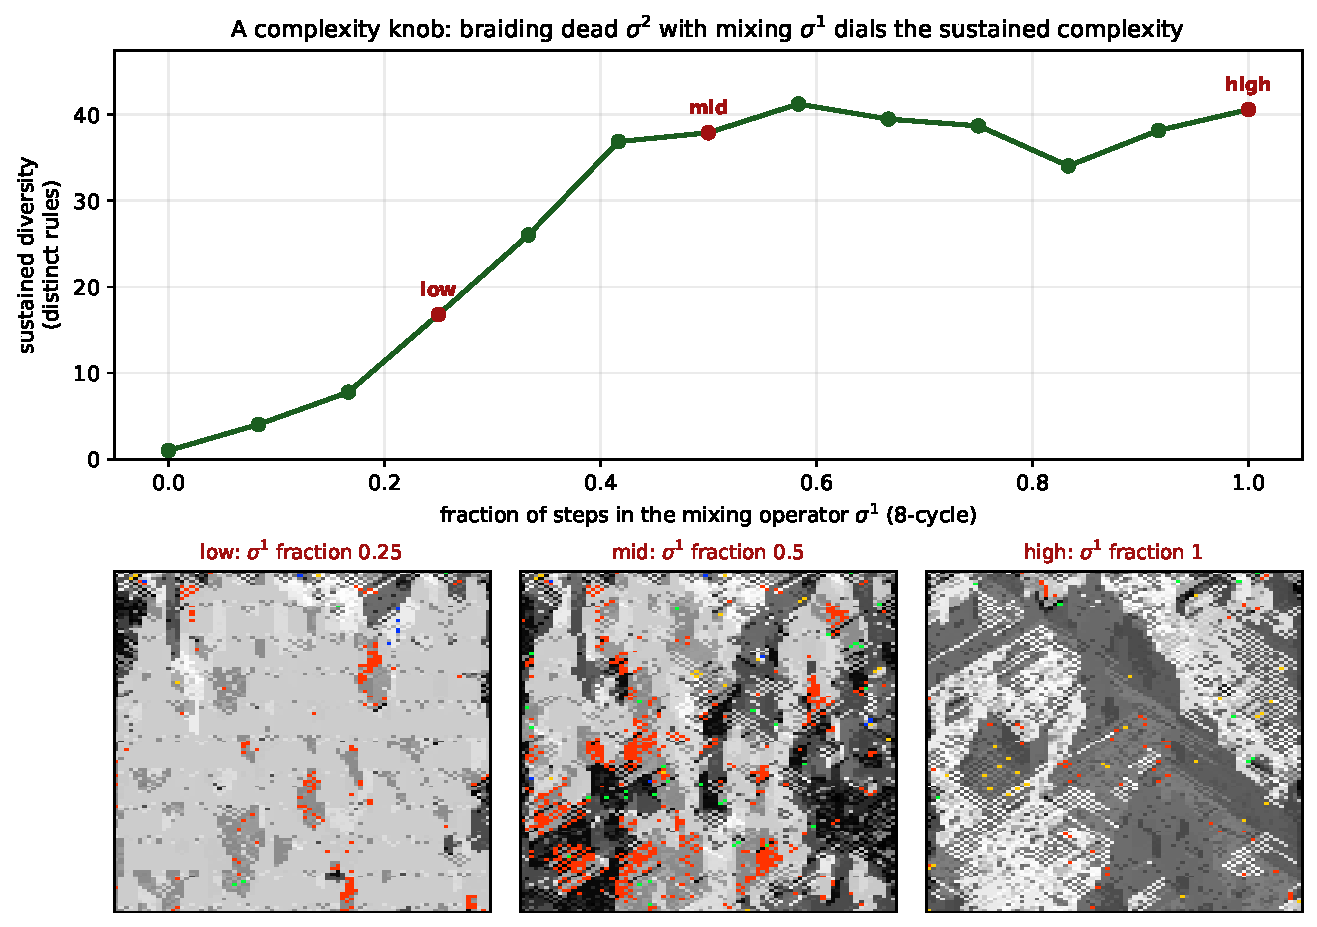
\includegraphics[width=\linewidth]{figures/knob.pdf}
\caption{\textbf{A diversity-control schedule.} Periodic 12-step schedules mix
the sustaining offset-$+1$ operator $\sigma^1$ with the collapsing offset-$+2$
operator $\sigma^2$. Mean late-window distinct-rule diversity (five seeds) rises
from $1.0$ with no $\sigma^1$ steps to a high-diversity plateau once its fraction
reaches roughly $0.4$. The three fields show fractions $0.25$, $0.50$, and $1.0$
at the same representative seed.}
\label{fig:knob}
\end{figure}

\begin{figure}[tb]
\centering
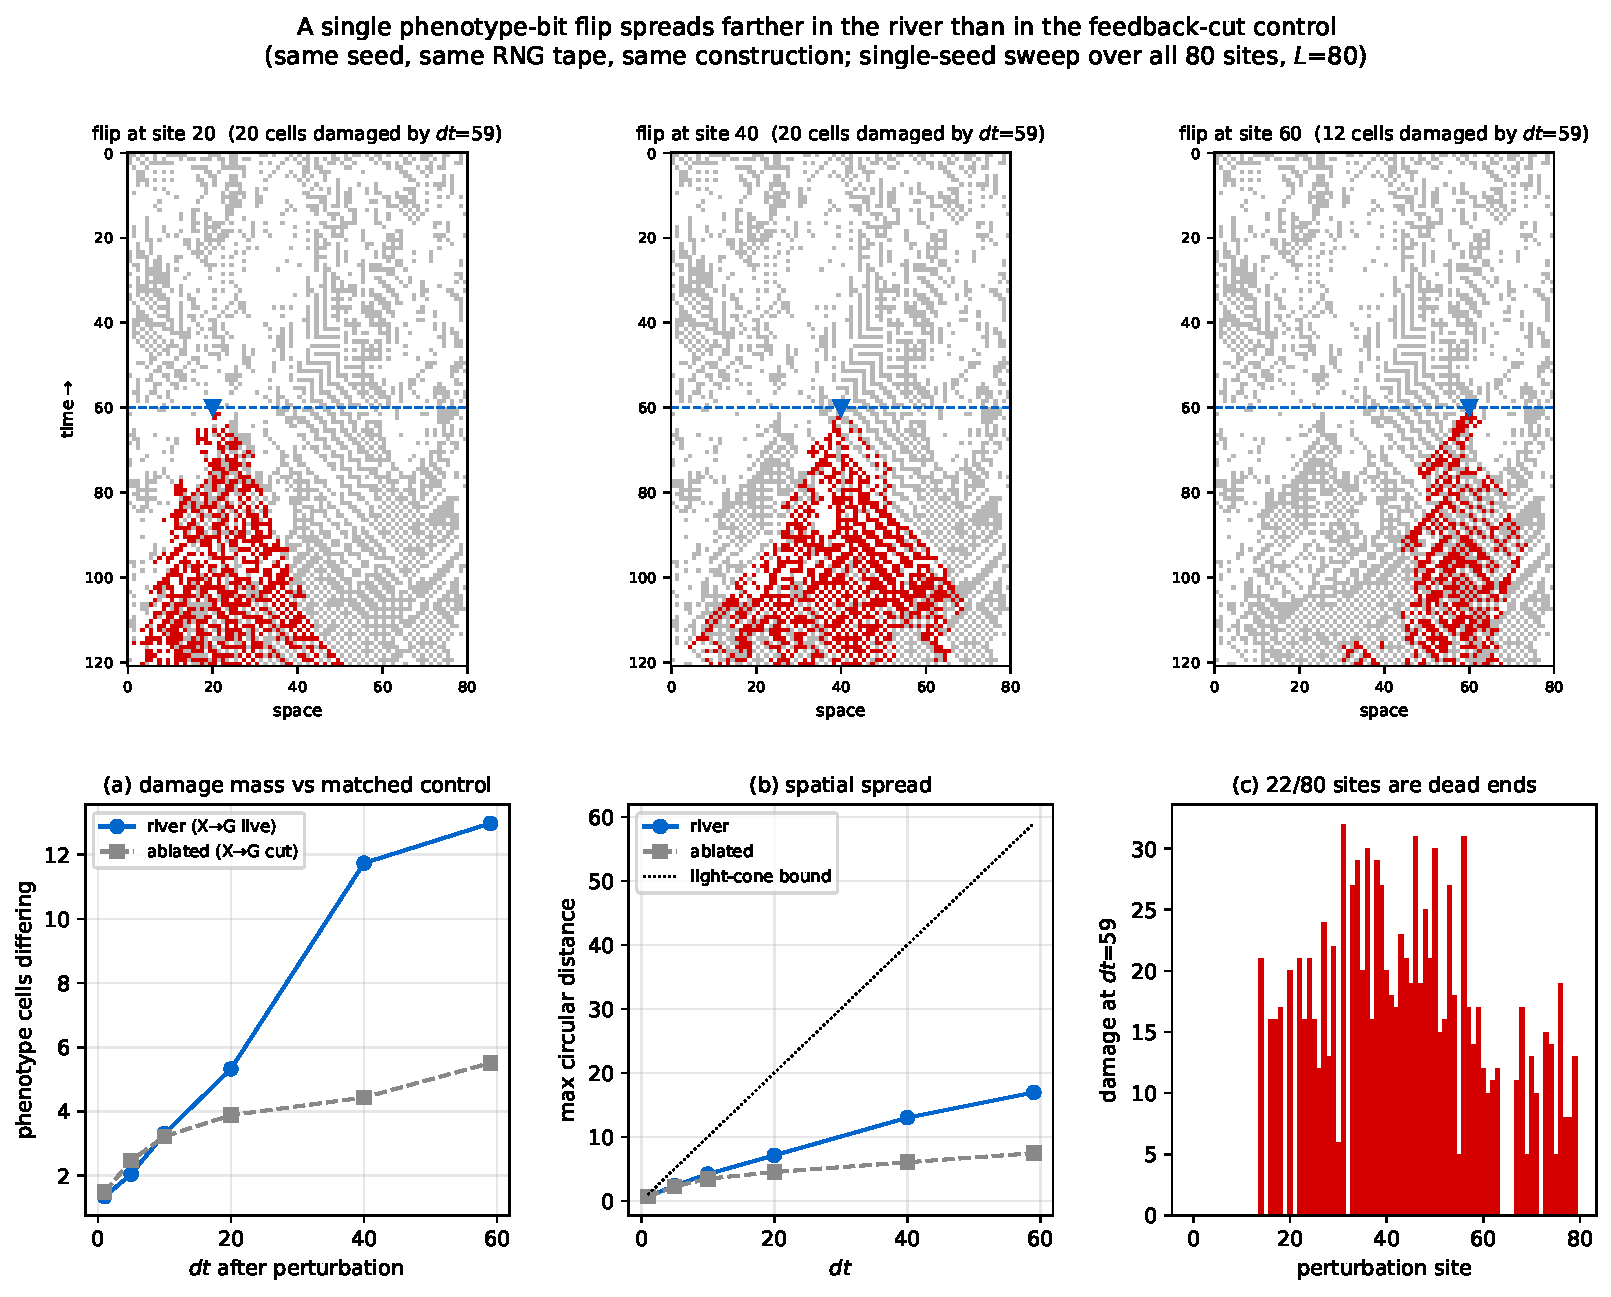
\includegraphics[width=0.94\linewidth]{figures/river_perturbation.pdf}
\caption{\textbf{Damage from a single phenotype flip.}
Live construction against its matched control, $L=80$, $t^{*}=60$, swept over all
$80$ sites; mass and spread at a sequence of horizons $dt$.}
\label{fig:river-perturbation}
\end{figure}

\begin{figure}[tb]
\centering
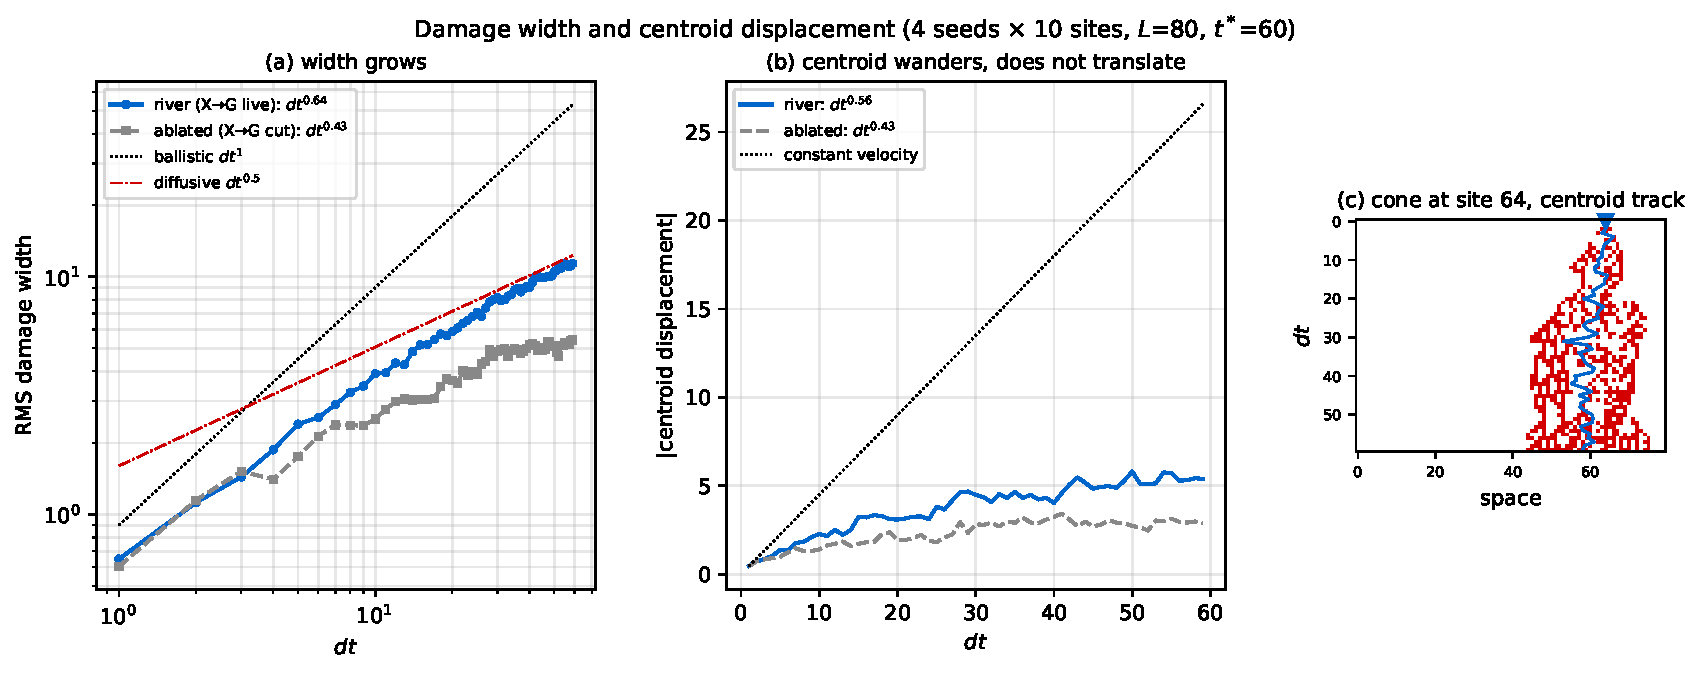
\includegraphics[width=0.94\linewidth]{figures/river_centroid.pdf}
\caption{\textbf{Damage width and centroid displacement.} \textbf{(a)}~damage width against $dt$,
log--log, with ballistic and diffusive references; \textbf{(b)}~centroid
displacement; \textbf{(c)}~a single cone with the centroid track overlaid. The
packet disperses while its centroid stays near the perturbation site. We do not
read this as excluding particle-like transport: under the same protocol rule
$110$, whose gliders support universal computation, gives $dt^{0.68}$ and
$dt^{0.73}$, so a random single-site perturbation does not produce a
fixed-width translating packet even where gliders certainly exist.}
\label{fig:river-centroid}
\end{figure}

\end{document}
